% A poster using beamerposter and the gemini theme with epfl colors.
% Beamerposter will let you create a poster in a single beamer frame
% using the columns and blocks from the beamer class.
% The color theme is adapted from Gemini's MIT scheme.

% use beamer as documentclass
\documentclass[final]{beamer}

% use the beamerposter package to create a poster
\usepackage[scale=1.4,orientation=portrait,size=a0]{beamerposter}
\usepackage{csquotes}
\usepackage[backend=biber,firstinits=true,maxbibnames=99,bibencoding=utf8,style=numeric]{biblatex}
\addbibresource{references.bib}
% make references small
\renewcommand*{\bibfont}{\scriptsize}

% use the gemini theme. 
\usetheme{gemini}
% If you prefer heavier fonts (looks nicer on screen):
% \setbeamerfont{block body}{family=\Lato}
% use the epfl color theme, defining epfl{dark}red, -{dark}green,  -light, -gray, and -dark
\usecolortheme{epfl}


\usepackage{booktabs}
\usepackage{amsmath}
\usepackage{graphicx}
\usepackage{tikz}
\usepackage{adjustbox}
\usepackage{qrcode}
\usepackage{wrapfig}
\usepackage{tikz-qtree}
\usepackage{pgfplots}
\pgfplotsset{compat=1.15}

% set OPG options
\tikzset{operation/.style={below,sloped,inner sep=1pt}} % with labels
% \tikzset{operation/.style={text opacity=0}} % without labels
\tikzset{external node/.style={}}
\tikzset{epsilon node/.style={}}
\tikzset{note node/.style={}}
\tikzset{every edge/.append style={line width=2.5pt}}
\tikzset{epsilon edge/.style={draw=epflgray}}
\tikzset{external edge/.style={draw=epflgray}}
% \tikzset{surface edge/.style={very thick}} % mark surface with thick edges
\tikzset{surface edge/.style={}} % don't mark surface

\newcommand{\generates}{\Rightarrow}
\newcommand{\dir}{\rightarrowtail}
\newcommand{\raga}{r\=aga}
\newcommand{\alap}{\=al\=ap}
\newcommand{\multani}{Mult\=an\=i}


\title{A Graph Grammar for\\North Indian Melodies}

\author{Christoph Finkensiep$^1$, Richard Widdess$^2$, and Martin Rohrmeier$^1$}

\institute{$^1$ École Polytechnique Fédérale de Lausanne\\$^2$ SOAS University of London}


\begin{document}

% header logos
\addtobeamertemplate{headline}{} 
{
  \begin{tikzpicture}[remember picture, overlay]
    \node [align=center,anchor=north west, inner sep=1.5cm]  at (current page.north west)
    {
      \includegraphics[height=5cm]{../logos/epfl/logo_print.pdf}
    };
  \end{tikzpicture}
}

\addtobeamertemplate{headline}{} 
{
  \begin{tikzpicture}[remember picture, overlay]
    \node [anchor=north east, inner sep=1.5cm]  at (current page.north east)
    {
      \includegraphics[height=5cm]{../logos/dcml/blue/with full name/DCML.pdf}
    };
  \end{tikzpicture}
}

\begin{frame}[t]

  \vfill
  
  \begin{columns}[t]
    \begin{column}{0.25\textwidth}
      \begin{block}{Basic Principles}
        Melodies of \alap\ performances can be understood as the result of \alert{recursive elaboration}
        of \alert{notes} and \alert{intervals}.

        \vspace{2em}
        
        \begin{tikzpicture}[overlay,font=\small]
          \node at (2.5,3.5) {step:};
          \node at (4.5,3.5) {1};
          \node at (8,3.5) {2};
          \node at (14,3.5) {3};
        \end{tikzpicture}
        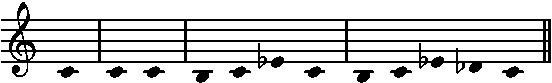
\includegraphics[width=\columnwidth]{figures/alap-phrase.pdf}
        \begin{center}
          \begin{small}
            A melody derived in three steps.
          \end{small}
        \end{center}

        \vspace{1em}
        
        Elaborations of notes include \alert{duplication} (1) and left or right \alert{neighbors} (2).
        Interval elaborations include \alert{passing notes} (3) and \alert{linear fills}.
        
      \end{block}
    \end{column}

    \begin{column}{0.25\textwidth}
      \begin{block}{Modes and Tonal Hierarchy}
        A mode is a scale together with a \alert{hierarchy of stability}
        among the scale degrees and restrictions on their \alert{movement direction}.

        \vspace{1em}

        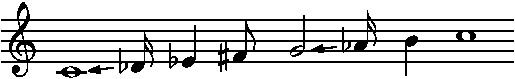
\includegraphics[width=\linewidth]{figures/scale.pdf}

        \begin{center}
          \begin{small}
            The tonal hiearchy of \raga\ \multani.
          \end{small}

          \vspace{1.3em}
            
          \setlength{\tabcolsep}{15pt}
          \begin{tabular}{lccccccc}
            \toprule
            pitch & 1 & \flat 2 & \flat 3 & \sharp 4 & 5 & \flat 6 & 7 \\
            \midrule
            direction & $\updownarrow$ & $\downarrow$ & $\updownarrow$ & $\updownarrow$
                                                     & $\updownarrow$ & $\downarrow$ & $\updownarrow$\\ 
            stability & 4 & 0 & 2 & 1 & 3 & 0 & 2 \\
            \toprule
          \end{tabular}
        \end{center}
        
        % Melodic elaboration respects both the hierarchical level and the directionality
        % of the scale degrees.
      \end{block}
    \end{column}

    \begin{column}{0.25\textwidth}
      \begin{block}{Distant Neighbors}
        Neighbors and passing notes can be \alert{non-adjacent}
        if they respect the tonal hierarchy of the mode.

        \vspace{0.5em}
        
        \begin{center}
          \begin{tikzpicture}
            \begin{axis}[
              ybar=0pt,
              /pgf/bar shift=0pt,
              bar width=25pt,
              symbolic x coords={{$7_\prime$},$1$,$\flat 2$,$\flat 3$,$\sharp 4$,$5$,$\flat 6$,$7$,$1'$,$\flat 2'$},
              xtick={{$7_\prime$},$1$,$\flat 2$,$\flat 3$,$\sharp 4$,$5$,$\flat 6$,$7$,$1'$,$\flat 2'$},
              ymajorticks=false,
              % axis y line=none,
              axis x line*=bottom,
              axis line style={draw=none},
              tick style={draw=none},
              height=7cm, width=\linewidth,
              ymin=0, ymax=5,% ylabel={\small hierarchical level}
              ]
              \addplot [draw=none,fill=epflred] coordinates {
                ($\flat 3$,3)
              };
              \addplot [draw=none,fill=epfldark] coordinates {
                ($1$,5)
                ($\sharp 4$,2)
                ($5$,4)
                ($1'$,5)
              };
              \addplot [draw=none,fill=epflgray] coordinates {
                ({$7_\prime$}, 3)
                ($\flat 2$, 1)
                ($\flat 6$, 1)
                ($7$, 3)
                ($\flat 2'$, 1)
              };
            \end{axis}
          \end{tikzpicture}

          \begin{small}
            The generalized neighbors of \flat 3 (dark).
          \end{small}
        \end{center}          
  
        A pitch $p_n$ is a \alert{generalized neighbor} of some pitch $p$
        if no pitch between $p$ and $p_n$ is more stable than $p$ and $p_n$.
      \end{block}
    \end{column}
  \end{columns}

  \vfill

  \centering
  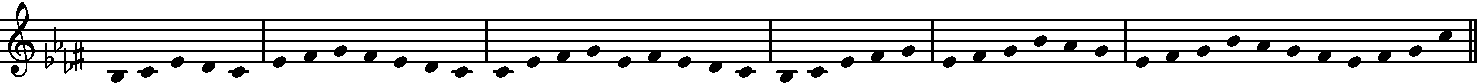
\includegraphics[width=0.9\textwidth]{figures/alap-example.pdf}
  
  \vspace{1cm}
  
  \begin{tikzpicture}[
    operation/.style={text opacity=0},
    every node/.style={circle,inner sep=5pt,font=\small},
    % xscale=0.325,yscale=0.6
    xscale=1.4,yscale=3
    ]
    % \node at (-3,0) {};
    \node[external node] (note0) at (0,0.0) {$\rtimes$};
\node[note node] (note9) at (1,-1.5) {$7_\prime$};
\node[note node] (note8) at (2,-1.0) {$1$};
\node[note node] (note10) at (3,-1.5) {$\flat3$};
\node[note node] (note11) at (4,-2.0) {$\flat2$};
\node[note node] (note2) at (5,-0.5) {$1$};
\node[epsilon node] (note5) at (6,-2.0) {$\varepsilon{}$};
\node[note node] (note14) at (7,-3.5) {$\flat3$};
\node[note node] (note12) at (8,-3.0) {$\sharp4$};
\node[note node] (note16) at (9,-4.5) {$5$};
\node[note node] (note15) at (10,-4.0) {$\sharp4$};
\node[note node] (note18) at (11,-5.0) {$\flat3$};
\node[note node] (note19) at (12,-5.0) {$\flat2$};
\node[note node] (note17) at (13,-4.5) {$1$};
\node[epsilon node] (note13) at (14,-3.5) {$\varepsilon{}$};
\node[note node] (note20) at (15,-4.0) {$1$};
\node[note node] (note21) at (16,-4.5) {$\flat3$};
\node[note node] (note22) at (17,-5.0) {$\sharp4$};
\node[note node] (note6) at (18,-2.5) {$5$};
\node[epsilon node] (note26) at (19,-5.0) {$\varepsilon{}$};
\node[note node] (note27) at (20,-5.5) {$\flat3$};
\node[note node] (note25) at (21,-4.5) {$\sharp4$};
\node[note node] (note24) at (22,-4.0) {$\flat3$};
\node[note node] (note28) at (23,-4.5) {$\flat2$};
\node[note node] (note23) at (24,-3.5) {$1$};
\node[epsilon node] (note7) at (25,-3.0) {$\varepsilon{}$};
\node[note node] (note34) at (26,-4.0) {$7_\prime$};
\node[note node] (note33) at (27,-3.5) {$1$};
\node[note node] (note35) at (28,-4.0) {$\flat3$};
\node[note node] (note36) at (29,-4.5) {$\sharp4$};
\node[note node] (note4) at (30,-1.5) {$5$};
\node[epsilon node] (note31) at (31,-3.0) {$\varepsilon{}$};
\node[note node] (note37) at (32,-3.5) {$\flat3$};
\node[note node] (note38) at (33,-4.0) {$\sharp4$};
\node[note node] (note30) at (34,-2.5) {$5$};
\node[note node] (note39) at (35,-3.5) {$7$};
\node[note node] (note40) at (36,-4.0) {$\flat6$};
\node[note node] (note32) at (37,-3.0) {$5$};
\node[epsilon node] (note29) at (38,-2.0) {$\varepsilon{}$};
\node[note node] (note43) at (39,-3.5) {$\flat3$};
\node[note node] (note44) at (40,-4.0) {$\sharp4$};
\node[note node] (note42) at (41,-3.0) {$5$};
\node[note node] (note41) at (42,-2.5) {$7$};
\node[note node] (note47) at (43,-4.0) {$\flat6$};
\node[note node] (note48) at (44,-4.0) {$5$};
\node[note node] (note49) at (45,-4.0) {$\sharp4$};
\node[note node] (note46) at (46,-3.5) {$\flat3$};
\node[note node] (note50) at (47,-4.0) {$\sharp4$};
\node[note node] (note45) at (48,-3.0) {$5$};
\node[note node] (note3) at (49,-1.0) {$1'$};
\node[external node] (note1) at (50,0.0) {$\ltimes$};
\draw (note0) edge[external edge] node[operation] {init} (note1);
\draw (note0) edge[external edge] node[operation] {dup$\to{}$} (note2);
\draw (note0) edge[external edge] node[operation] {nb$\to{}$} (note8);
\draw (note0) edge[external edge,surface edge] node[operation] {} (note9);
\draw (note2) edge[external edge] node[operation] {$\leftarrow{}$nb} (note1);
\draw (note2) edge[] node[operation] {pass} (note3);
\draw (note2) edge[] node[operation] {split} (note4);
\draw (note2) edge[epsilon edge,surface edge] node[operation] {} (note5);
\draw (note3) edge[external edge,surface edge] node[operation] {} (note1);
\draw (note4) edge[] node[operation] {split} (note3);
\draw (note4) edge[epsilon edge] node[operation] {$\leftarrow{}$dup} (note29);
\draw (note4) edge[] node[operation] {split} (note30);
\draw (note4) edge[epsilon edge,surface edge] node[operation] {} (note31);
\draw (note5) edge[epsilon edge] node[operation] {dup$\to{}$} (note4);
\draw (note5) edge[epsilon edge] node[operation] {nb$\to{}$} (note6);
\draw (note5) edge[epsilon edge] node[operation] {nb$\to{}$} (note12);
\draw (note5) edge[epsilon edge,surface edge] node[operation] {} (note14);
\draw (note6) edge[] node[operation] {split} (note4);
\draw (note6) edge[epsilon edge] node[operation] {$\leftarrow{}$nb} (note7);
\draw (note6) edge[] node[operation] {pass} (note23);
\draw (note6) edge[] node[operation] {pass} (note24);
\draw (note6) edge[] node[operation] {split} (note25);
\draw (note6) edge[epsilon edge,surface edge] node[operation] {} (note26);
\draw (note7) edge[epsilon edge] node[operation] {nb$\to{}$} (note4);
\draw (note7) edge[epsilon edge] node[operation] {nb$\to{}$} (note33);
\draw (note7) edge[epsilon edge,surface edge] node[operation] {} (note34);
\draw (note8) edge[] node[operation] {nb$\to{}$} (note2);
\draw (note8) edge[surface edge] node[operation] {} (note10);
\draw (note9) edge[surface edge] node[operation] {} (note8);
\draw (note10) edge[] node[operation] {pass} (note2);
\draw (note10) edge[surface edge] node[operation] {} (note11);
\draw (note11) edge[surface edge] node[operation] {} (note2);
\draw (note12) edge[] node[operation] {split} (note6);
\draw (note12) edge[epsilon edge] node[operation] {$\leftarrow{}$dup} (note13);
\draw (note12) edge[] node[operation] {nb$\to{}$} (note15);
\draw (note12) edge[surface edge] node[operation] {} (note16);
\draw (note13) edge[epsilon edge] node[operation] {nb$\to{}$} (note6);
\draw (note13) edge[epsilon edge,surface edge] node[operation] {} (note20);
\draw (note14) edge[surface edge] node[operation] {} (note12);
\draw (note15) edge[epsilon edge] node[operation] {$\leftarrow{}$nb} (note13);
\draw (note15) edge[] node[operation] {fill} (note17);
\draw (note15) edge[surface edge] node[operation] {} (note18);
\draw (note16) edge[surface edge] node[operation] {} (note15);
\draw (note17) edge[epsilon edge,surface edge] node[operation] {} (note13);
\draw (note18) edge[surface edge] node[operation] {} (note19);
\draw (note19) edge[surface edge] node[operation] {} (note17);
\draw (note20) edge[] node[operation] {pass} (note6);
\draw (note20) edge[surface edge] node[operation] {} (note21);
\draw (note21) edge[] node[operation] {pass} (note6);
\draw (note21) edge[surface edge] node[operation] {} (note22);
\draw (note22) edge[surface edge] node[operation] {} (note6);
\draw (note23) edge[epsilon edge,surface edge] node[operation] {} (note7);
\draw (note24) edge[] node[operation] {pass} (note23);
\draw (note24) edge[surface edge] node[operation] {} (note28);
\draw (note25) edge[surface edge] node[operation] {} (note24);
\draw (note26) edge[epsilon edge] node[operation] {nb$\to{}$} (note25);
\draw (note26) edge[epsilon edge,surface edge] node[operation] {} (note27);
\draw (note27) edge[surface edge] node[operation] {} (note25);
\draw (note28) edge[surface edge] node[operation] {} (note23);
\draw (note29) edge[epsilon edge] node[operation] {nb$\to{}$} (note3);
\draw (note29) edge[epsilon edge] node[operation] {nb$\to{}$} (note41);
\draw (note29) edge[epsilon edge] node[operation] {nb$\to{}$} (note42);
\draw (note29) edge[epsilon edge,surface edge] node[operation] {} (note43);
\draw (note30) edge[epsilon edge] node[operation] {$\leftarrow{}$dup} (note29);
\draw (note30) edge[] node[operation] {nb$\to{}$} (note32);
\draw (note30) edge[surface edge] node[operation] {} (note39);
\draw (note31) edge[epsilon edge] node[operation] {nb$\to{}$} (note30);
\draw (note31) edge[epsilon edge,surface edge] node[operation] {} (note37);
\draw (note32) edge[epsilon edge,surface edge] node[operation] {} (note29);
\draw (note33) edge[] node[operation] {pass} (note4);
\draw (note33) edge[surface edge] node[operation] {} (note35);
\draw (note34) edge[surface edge] node[operation] {} (note33);
\draw (note35) edge[] node[operation] {pass} (note4);
\draw (note35) edge[surface edge] node[operation] {} (note36);
\draw (note36) edge[surface edge] node[operation] {} (note4);
\draw (note37) edge[] node[operation] {pass} (note30);
\draw (note37) edge[surface edge] node[operation] {} (note38);
\draw (note38) edge[surface edge] node[operation] {} (note30);
\draw (note39) edge[] node[operation] {pass} (note32);
\draw (note39) edge[surface edge] node[operation] {} (note40);
\draw (note40) edge[surface edge] node[operation] {} (note32);
\draw (note41) edge[] node[operation] {nb$\to{}$} (note3);
\draw (note41) edge[] node[operation] {nb$\to{}$} (note45);
\draw (note41) edge[] node[operation] {fill} (note46);
\draw (note41) edge[surface edge] node[operation] {} (note47);
\draw (note42) edge[surface edge] node[operation] {} (note41);
\draw (note43) edge[] node[operation] {pass} (note42);
\draw (note43) edge[surface edge] node[operation] {} (note44);
\draw (note44) edge[surface edge] node[operation] {} (note42);
\draw (note45) edge[surface edge] node[operation] {} (note3);
\draw (note46) edge[] node[operation] {pass} (note45);
\draw (note46) edge[surface edge] node[operation] {} (note50);
\draw (note47) edge[surface edge] node[operation] {} (note48);
\draw (note48) edge[surface edge] node[operation] {} (note49);
\draw (note49) edge[surface edge] node[operation] {} (note46);
\draw (note50) edge[surface edge] node[operation] {} (note45);

  \end{tikzpicture}

  \begin{small}
    Selected phrases, in order of performance,
    from the ascending part of an \alap\ in \raga\ \multani,
    recorded by the sitarist Dharambir Singh.
  \end{small}
  
  \vfill
  
  \begin{columns}[t]
    
    \begin{column}{0.25\textwidth}
      \begin{block}{Formal Representation}
        Since both notes and intervals are elaborated,
        melodies are represented as graphs with \alert{notes as nodes}
        and \alert{intervals as edges}.
        The elaboration operations then form an edge-replacement \alert{graph grammar}.
        
        Interval elaborations replace an edge with a new subgraph:
        \[ (n_1 \to n_2) \longrightarrow (n_1 \to n' \to n_2) \]
        Note elaboration also replace edges but consider only one of the nodes:
        \[ (n_1 \to *) \longrightarrow (n_1 \to n' \to *) \]
        Independent parts of the graph can be separated explicitly
        by introducing an \alert{empty node}:
        \[ (n_1 \to n_2) \longrightarrow (n_1 \to \varepsilon \to n_2) \]

        Another advantage of graphs is that they can capture more complex structures
        such as \alert{polyphonic networks}.
      \end{block}
    \end{column}

    \begin{column}{0.25\textwidth}
      \begin{block}{Graphical Notation}
        Since the graph of a monophonic melody is linear,
        its derivation can be visualized by an \alert{outerplanar graph}
        \autocite{YustGeometryMelodicHarmonic2009},
        where each polygon represents an edge replacement.

        \begin{tikzpicture}[
          operation/.append style={inner sep=3pt,font=\small},
          every edge/.append style={->,draw=black},
          scale=2.8
          ]
          \node[external node] (note0) at (0,0.0) {$\rtimes$};
          \node[note node] (note5) at (1,-1.5) {$7_\prime$};
          \node[note node] (note3) at (2,-1.0) {$1$};
          \node[epsilon node] (note4) at (3,-1.5) {$\varepsilon{}$};
          \node[note node] (note6) at (4,-2.0) {$\flat3$};
          \node[note node] (note7) at (5,-2.5) {$\flat2$};
          \node[note node] (note2) at (6,-0.5) {$1$};
          \node[external node] (note1) at (7,0.0) {$\ltimes$};
          \draw (note0) edge[external edge] node[operation,pos=0.8] {init} (note1);
          \draw (note0) edge[external edge] node[operation] {dup$\to{}$} (note2);
          \draw (note0) edge[external edge] node[operation,pos=0.6] {nb$\to{}$} (note3);
          \draw (note0) edge[external edge,surface edge] node[operation] {} (note5);
          \draw (note2) edge[external edge,surface edge] node[operation] {} (note1);
          \draw (note3) edge[] node[operation,pos=0.3] {split} (note2);
          \draw (note3) edge[epsilon edge,surface edge] node[operation] {} (note4);
          \draw (note4) edge[epsilon edge] node[operation,pos=0.4] {nb$\to{}$} (note2);
          \draw (note4) edge[epsilon edge,surface edge] node[operation] {} (note6);
          \draw (note5) edge[surface edge] node[operation] {} (note3);
          \draw (note6) edge[] node[operation,pos=0.4] {pass} (note2);
          \draw (note6) edge[surface edge] node[operation] {} (note7);
          \draw (note7) edge[surface edge] node[operation] {} (note2);
        \end{tikzpicture}
        
        Indepencene is indicated by $\varepsilon$-nodes.
        Adjacent edges are shown in light gray,
        revealing the differences between note and interval elaborations.
        
      \end{block}

      \begin{block}{References}
        \printbibliography
      \end{block}
    \end{column}
    
    \begin{column}{0.25\textwidth}

      \begin{block}{Funding and Paper Link}
        \begin{wrapfigure}{l}{0.3\textwidth}
          \begin{center}
            \qrcode[height=0.25\textwidth]{http://archives.ismir.net/ismir2019/paper/000055.pdf}
          \end{center}
        \end{wrapfigure}
        \small
        The research presented on this poster is generously supported
        by the Volkswagen Foundation and Claude Latour.
        This project has received funding from the European Research Council (ERC)
        under the European Union's Horizon 2020 research and innovation programme
        under grant agreement No 760081 – PMSB.
        We thank Dharambir Singh for the permission to use his recording of an
        \alap\ in \raga\ \multani.

        \begin{adjustbox}{valign=m}
        \includegraphics[width=0.5\textwidth]{../logos/epfl/logo_print.pdf}
        
\includegraphics[width=0.5\textwidth]{figures/soas.jpg}
        \end{adjustbox}

        \includegraphics[width=\textwidth]{../logos/vw/vw.pdf}

        \begin{adjustbox}{valign=m}
        \includegraphics[width=0.5\textwidth,,trim=0 -2cm 0 0]{../logos/erc/flag.pdf}
        \includegraphics[width=0.5\textwidth]{../logos/erc/erc.pdf}
        \end{adjustbox}

        
      \end{block}
    \end{column}
    
  \end{columns}

  \vfill
  
\end{frame} % End of the enclosing frame

\end{document}
% Local Variables:
% TeX-engine: luatex
% TeX-command-extra-options: "-shell-escape"
% End:
